% Layout proof only: does not modify or include the manuscript source.
\documentclass[aps,prb,10pt,twocolumn,superscriptaddress,floatfix]{revtex4-2}
\usepackage{amsmath,amssymb,graphicx,capt-of,xcolor}
\usepackage[colorlinks=true]{hyperref}
\newsavebox{\figureblock}
\newdimen\remainingroom
\begin{document}
\thispagestyle{empty}
\begin{lrbox}{\figureblock}
\begin{minipage}{\columnwidth}
\centering
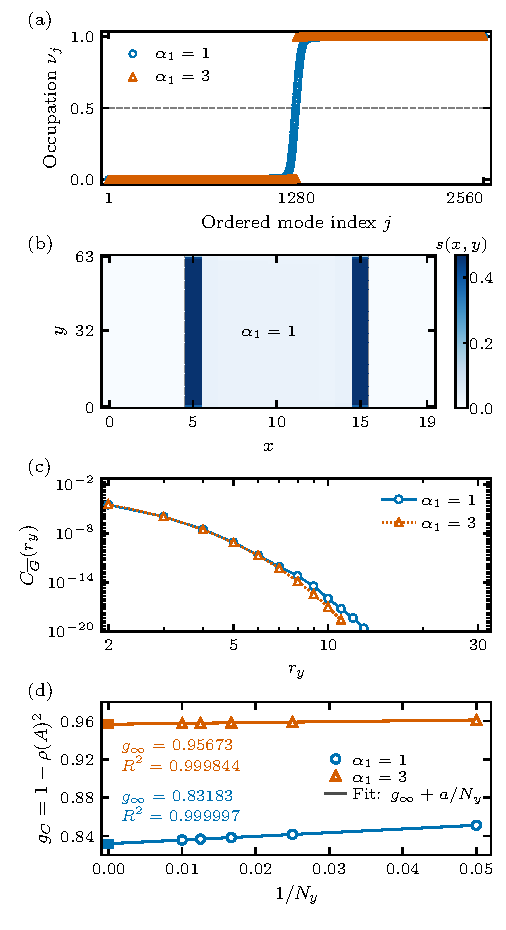
\includegraphics[width=\columnwidth]{Mean_channel_four_rows.pdf}
\captionof{figure}{Outcome-averaged hard-wall channel.
(a) Endpoint occupation spectra for $\alpha_1=1,3$.
(b) Full-system entropy contour $s(x,y)$ for $\alpha_1=1$, in nats per unit cell.
(c) Squared averaged correlator.
Panels (a)--(c) use the untwirled endpoints at cycle 128, starting from maximal mixing,
with $N_x=20$, $N_y=64$ and $n_{\mathrm{shell}}=1$; outcomes are averaged analytically.
(d) Channel gap $g_C=1-\rho(A)^2$ at fixed $N_x=20$ and varying $N_y$;
lines are the saved $g_\infty+a/N_y$ fits.
This caption is for layout assessment only.}
\end{minipage}
\end{lrbox}
\remainingroom=\dimexpr\textheight-\ht\figureblock-\dp\figureblock\relax
\typeout{LAYOUT-COLUMN-WIDTH: \the\columnwidth}
\typeout{LAYOUT-TEXT-HEIGHT: \the\textheight}
\typeout{LAYOUT-FIGURE-AND-CAPTION: \the\dimexpr\ht\figureblock+\dp\figureblock\relax}
\typeout{LAYOUT-REMAINING-ROOM: \the\remainingroom}
\noindent\begin{minipage}{\columnwidth}
\usebox{\figureblock}\par\medskip
\noindent\fcolorbox{gray}{gray!6}{%
\parbox[c][0.75in][c]{\dimexpr\columnwidth-2\fboxsep-2\fboxrule\relax}{%
\centering\color{gray}Main text continues here.\par
\smallskip\small This box marks available text space;\par
no manuscript prose has been changed.}}
\end{minipage}
\end{document}
